\documentclass[theme=teal]{khmermath}
\usepackage{needspace}

\geometry{left=0.85cm, right=0.85cm, top=0.75cm, bottom=1.5cm, footskip=0.7cm}
\usepackage{colortbl}
\usepackage{tikz}
\usetikzlibrary{calc,shapes,arrows,intersections,through,backgrounds,shadows,decorations.pathmorphing,angles,quotes}

% -------------------------------------------------------------------------
% Korean Math Textbook Style Color Palette & Macros
% -------------------------------------------------------------------------
\definecolor{koreaTeal}{RGB}{0, 150, 155}       % Primary Header Teal/Cyan
\definecolor{koreaDarkTeal}{RGB}{0, 105, 110}   % Dark Teal Accent
\definecolor{koreaBeige}{RGB}{247, 244, 237}     % Concept Sidebar Beige (#F7F4EE)
\definecolor{koreaBeigeBorder}{RGB}{225, 218, 205}
\definecolor{koreaOrange}{RGB}{235, 115, 30}     % Problem Number Orange
\definecolor{koreaBlue}{RGB}{35, 110, 190}      % Standard Blue
\definecolor{koreaPurple}{RGB}{125, 50, 160}    % Purple Accent
\definecolor{koreaNumber}{RGB}{115, 125, 135}   % Problem Number Gray
\definecolor{koreaYellow}{RGB}{255, 246, 175}   % Yellow Highlight Tint

\definecolor{brandNavy}{RGB}{0, 105, 110}
\definecolor{brandBlue}{RGB}{0, 150, 155}
\definecolor{brandLightBlue}{RGB}{247, 244, 237}
\definecolor{brandCrimson}{RGB}{195, 35, 60}
\definecolor{brandCoral}{RGB}{235, 80, 75}
\definecolor{brandGold}{RGB}{215, 130, 10}
\definecolor{brandGoldBg}{RGB}{255, 252, 242}
\definecolor{brandTeal}{RGB}{0, 150, 155}
\definecolor{brandTealBg}{RGB}{244, 252, 250}
\definecolor{subtleGray}{RGB}{246, 251, 249}
\definecolor{cardBorder}{RGB}{220, 212, 198}

% Custom Header & Footer setup (Korean Textbook Style)
\usepackage{fancyhdr}
\pagestyle{fancy}
\fancyhf{}
\renewcommand{\headrulewidth}{0pt}
\renewcommand{\footrule}{\color{koreaTeal!60}\hrule height 0.6pt\vspace{3pt}}

\fancyfoot[L]{%
  \fontsize{8.5}{8.5}\selectfont\kml \color{koreaNumber}\textbf{\thepage}\ \vline\ \color{koreaDarkTeal}\textbf{មេរៀនទី ១០ ៖ សមីការនៃបន្ទាត់}%
}
\fancyfoot[C]{%
  \fontsize{8.5}{8.5}\selectfont\kby \color{koreaDarkTeal}\textbf{\ding{72}\ បង្រៀនដោយ ៖ \textcolor{koreaDarkTeal}{ក្រូត រស្មី}\ \ding{72}}%
}
\fancyfoot[R]{%
  \fontsize{8.5}{8.5}\selectfont\kby \color{koreaDarkTeal}\textbf{ Telegram: \textcolor{brandCrimson}{070897540}}\ \vline\ \color{koreaNumber}\textbf{\thepage}%
}

% Korean Header Banner
\newcommand{\koreanheader}[2]{%
  \noindent%
  \begin{tikzpicture}[x=1cm, y=1cm]
    \fill[koreaTeal, rounded corners=12pt] (0, 0.1) -- (0, 0.95) -- (3.8, 0.95) [rounded corners=0pt] -- (4.4, 0.1) -- cycle;
    \node[white, font=\fontsize{11}{11}\selectfont\kml\bfseries] at (1.9, 0.52) {#1};
    \node[anchor=west, font=\fontsize{17}{17}\selectfont\kml\bfseries, color=koreaDarkTeal] at (4.6, 0.42) {#2};
    \node[anchor=east, font=\fontsize{8.5}{8.5}\selectfont\kby, color=gray!80] at (19.2, 0.48) {$>$ ក្លឹបសិក្សាគណិតវិទ្យា ភី ស៊ី​ អឹម};
  \end{tikzpicture}%
  \vspace{3pt}%
}

% Yellow Formula Highlight Box
\newcommand{\koreahl}[1]{\colorbox{koreaYellow}{\fontsize{8.5}{8.5}\selectfont\textbf{#1}}}

% General Rule Box (Teal/Emerald Theme - ជាទូទៅ)
\newtcolorbox{khboxorange}[1][]{
  enhanced,
  colframe=brandNavy!40,
  colback=brandLightBlue,
  boxrule=0.7pt,
  arc=5.0pt,
  borderline west={3.5pt}{0pt}{brandNavy},
  drop fuzzy shadow=brandNavy!15,
  left=9pt, right=9pt, top=5pt, bottom=5pt,
  title={\fontsize{9.5}{9.5}\selectfont\kml\color{white}\ding{72}\ ជាទូទៅ},
  coltitle=white,
  colbacktitle=brandNavy,
  boxed title style={
    boxrule=0pt,
    arc=3.5pt,
    left=7pt, right=7pt, top=2.5pt, bottom=2.5pt
  },
  attach boxed title to top left={yshift*=-\tcboxedtitleheight/2, xshift=12pt},
  #1
}

% Example / Card Item Box
\newtcolorbox{khcard}[1][]{
  enhanced,
  colframe=cardBorder,
  colback=white,
  boxrule=0.7pt,
  arc=3.5pt,
  left=6pt, right=6pt, top=4pt, bottom=4pt,
  #1
}

% Section & Subsection Macros
\newcommand{\khsection}[2]{%
  \Needspace*{3.5cm}%
  \vspace{3pt}%
  \noindent%
  \begin{tikzpicture}
    \fill[rounded corners=5pt, brandNavy!8] (0,0) rectangle (19.3, 0.68);
    \fill[rounded corners=4pt, brandNavy] (0.06, 0.06) rectangle (0.62, 0.62);
    \node[white, font=\fontsize{10}{10}\selectfont\bfseries] at (0.34, 0.34) {#1};
    \fill[brandGold, rounded corners=1pt] (0.72, 0.15) rectangle (0.76, 0.53);
    \node[anchor=west, font=\fontsize{11.5}{11.5}\selectfont\kml, color=brandCrimson] at (0.83, 0.34) {\textbf{#2}};
  \end{tikzpicture}%
  \vspace{2pt}%
}

\newcommand{\khsubsection}[2]{%
  \Needspace*{3.2cm}%
  \vspace{2pt}%
  \noindent%
  \begin{tikzpicture}[baseline=(sub.base)]
    \node[rounded corners=3.5pt, fill=brandBlue!12, draw=brandBlue!35, line width=0.5pt, text=brandNavy, font=\fontsize{9}{9}\selectfont\kml\bfseries, inner sep=3pt] (sub) at (0,0) {#1};
    \node[anchor=west, font=\fontsize{10}{10}\selectfont\kml\bfseries, color=brandNavy] at (sub.east) {\ \ #2};
  \end{tikzpicture}%
  \vspace{1.5pt}%
}

\def\splitnum#1#2{%
  \color{koreaNumber!65}#1\color{koreaOrange}#2%
}
\newcommand{\koreannum}[1]{%
  \ifstrempty{#1}{}{%
    \mbox{%
      \fontsize{15}{15}\selectfont\bfseries%
      \ifnum#1<10\relax%
        \color{koreaNumber!65}0\color{koreaOrange}#1%
      \else%
        \expandafter\splitnum#1%
      \fi%
    }\,\ %
  }%
}

% Khmer sub-question badge
\newcommand{\khlabel}[1]{%
  \tikz[baseline=-0.6ex]{%
    \node[fill=brandCrimson, rounded corners=3pt, inner sep=2pt, minimum width=1.3em, minimum height=1.28em, text=white, font=\kml\fontsize{7.5}{7.5}\selectfont, align=center] (lbl) {\raisebox{0.2pt}{#1}};%
  }\,\ %
}
\newcommand{\exhead}[1]{\koreannum{#1}}

\setlength{\parindent}{0pt}
\setlength{\parskip}{2.5pt}
\setlength{\columnsep}{16pt}
\setlength{\columnseprule}{0.5pt}
\def\columnseprulecolor{\color{koreaTeal!40}}

\begin{document}

% =========================================================================
% PAGE 1: ១.១ ការសង់បន្ទាត់តាមតារាងតម្លៃលេខ
% =========================================================================
\koreanheader{មេរៀនទី ១០}{សមីការនៃបន្ទាត់}

\khsection{១}{ការសង់បន្ទាត់}

\khsubsection{១.១}{ការសង់បន្ទាត់តាមតារាងតម្លៃលេខ}

\begin{khcard}
  \begin{minipage}[c]{0.59\textwidth}
    \textbf{\color{brandNavy}របៀបសង់បន្ទាត់ $y = 2x - 3$ តាម ២ ចំណុច ៖}\\[1.5pt]
    \textbf{\color{brandCrimson}\ding{228} ជំហានទី ១ ៖ កំណត់តារាងតម្លៃលេខ (ជ្រើសយក ២ ចំណុច)}
    \begin{itemize}[leftmargin=10pt, itemsep=1.5pt, topsep=1.5pt, parsep=0pt]
      \item[\color{brandNavy}\textbullet] បើ $x = 0 \Rightarrow y = 2(0) - 3 = -3 \longrightarrow \text{ចំណុច } A(0, -3)$
      \item[\color{brandNavy}\textbullet] បើ $x = 2 \Rightarrow y = 2(2) - 3 = 1 \longrightarrow \text{ចំណុច } B(2, 1)$
    \end{itemize}
    \vspace{1pt}
    \centering
    \renewcommand{\arraystretch}{1.1}
    \begin{tabular}{|c|c|c|}
      \hline
      \rowcolor{koreaTeal!15}
      \textbf{\boldmath$x$} & $0$ & $2$ \\
      \hline
      \textbf{\boldmath$y$} & $-3$ & $1$ \\
      \hline
      \rowcolor{koreaBeige}
      \textbf{ចំណុច} & $A(0,-3)$ & $B(2,1)$ \\
      \hline
    \end{tabular}
    \\[3pt]
    \raggedright
    \textbf{\color{brandCrimson}\ding{228} ជំហានទី ២ ៖ ដៅចំណុច និងគូសបន្ទាត់}
    \begin{itemize}[leftmargin=10pt, itemsep=1.5pt, topsep=1.5pt, parsep=0pt]
      \item[\circled{1}] ដៅចំណុច $A(0, -3)$ និង $B(2, 1)$ លើប្លង់កូអរដោនេ
      \item[\circled{2}] \textbf{បកស្រាយលើរូប ៖} $a = \frac{\Delta y}{\Delta x} = \frac{1 - (-3)}{2 - 0} = \frac{4}{2} = 2$
      \begin{itemize}[leftmargin=8pt, itemsep=1pt, topsep=1pt, parsep=0pt]
        \item[\color{brandGold}\tiny\ding{108}] \textbf{\boldmath$\Delta x = +2$} ៖ ពី $x=0$ រំកិលទៅស្ដាំ $2$ ឯកតា (តាមដេក)
        \item[\color{brandCrimson}\tiny\ding{108}] \textbf{\boldmath$\Delta y = +4$} ៖ ពី $y=-3$ រំកិលឡើងលើ $4$ ឯកតា (តាមឈរ)
      \end{itemize}
      \item[\circled{3}] គូសបន្ទាត់ត្រង់កាត់តាមពីរចំណុច $A$ និង $B$ បានបន្ទាត់ $y = 2x - 3$ ។
    \end{itemize}
  \end{minipage}\hfill
  \begin{minipage}[c]{0.40\textwidth}
    \centering
    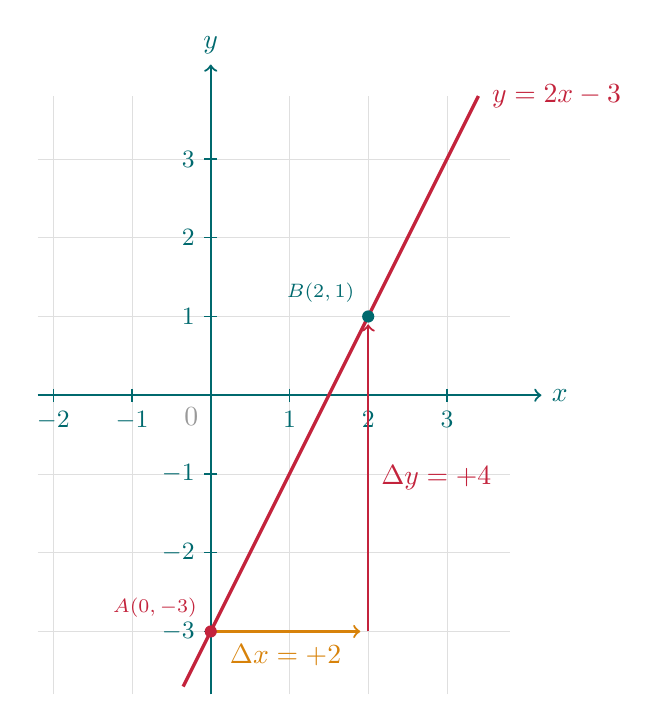
\begin{tikzpicture}[scale=1]
      \draw[very thin, gray!25, step=1] (-2.2,-3.8) grid (3.8,3.8);
      \draw[->, thick, koreaDarkTeal] (-2.2,0) -- (4.2,0) node[right, font=\bfseries] {$x$};
      \draw[->, thick, koreaDarkTeal] (0,-3.8) -- (0,4.2) node[above, font=\bfseries] {$y$};
      \node[below left=1pt, color=gray!80] at (0,0) {$0$};
      
      % Ticks
      \foreach \x in {-2,-1,1,2,3}
        \draw[koreaDarkTeal] (\x,0.08) -- (\x,-0.08) node[below, font=\fontsize{9}{5.5}\selectfont] {$\x$};
      \foreach \y in {-3,-2,-1,1,2,3}
        \draw[koreaDarkTeal] (0.08,\y) -- (-0.08,\y) node[left, font=\fontsize{9}{5.5}\selectfont] {$\y$};
      
      % Coordinates
      \coordinate (A) at (0,-3);
      \coordinate (B) at (2,1);
      
      % Slope step arrows & annotations
      \draw[->, thick, color=brandGold] (0,-3) -- (1.9,-3) node[midway, below=1pt, font=\bfseries, text=brandGold] {$\Delta x = +2$};
      \draw[->, thick, color=brandCrimson] (2,-3) -- (2,0.9) node[midway, right=1pt, font=\bfseries, text=brandCrimson] {$\Delta y = +4$};
      
      % Line
      \draw[very thick, color=brandCrimson] (-0.35,-3.7) -- (3.4,3.8) node[right=1pt, text=brandCrimson] {$y = 2x - 3$};
      
      % Highlight Points with Names
      \fill[brandCrimson] (A) circle (2.2pt);
      \node[above left=1.5pt, font=\scriptsize\bfseries, text=brandCrimson] at (A) {$A(0,-3)$};
      
      \fill[brandNavy] (B) circle (2.2pt);
      \node[above left=1.5pt, font=\scriptsize\bfseries, text=brandNavy] at (B) {$B(2,1)$};
    \end{tikzpicture}
  \end{minipage}
\end{khcard}

\vspace{2.5pt}

\begin{khboxorange}
  \begin{itemize}[leftmargin=12pt, itemsep=2pt, topsep=1pt, parsep=0pt]
    \item[\color{brandNavy}\ding{228}] \textbf{សមីការទូទៅ ៖} \ \koreahl{$y = ax + b$} \ ($a$ ជា\textbf{មេគុណប្រាប់ទិស} ឬកម្រិតចោត, $b$ ជា\textbf{អរដោនេដើម} ឬកាត់អ័ក្ស $y'y$ ត្រង់ $(0, b)$) ។
    \item[\color{brandCrimson}\ding{228}] \textbf{មេគុណប្រាប់ទិសនៃបន្ទាត់កាត់តាមពីរចំណុច} $A(x_1, y_1)$ និង $B(x_2, y_2)$ ដែល $x_1 \neq x_2$ ៖
    \begin{equation*}
      \koreahl{$a = \frac{\Delta y}{\Delta x} = \frac{y_2 - y_1}{x_2 - x_1} = \frac{\text{បម្រែបម្រួលកម្ពស់ } y}{\text{បម្រែបម្រួលចម្ងាយ } x}$}
    \end{equation*}
  \end{itemize}
\end{khboxorange}

\vspace{2pt}

\noindent
\exhead{1} \textbf{ចូរសង់សមីការបន្ទាត់នីមួយៗខាងក្រោម ៖}
\begin{center}
\renewcommand{\arraystretch}{1.2}
\begin{tabular}{p{4.4cm}p{4.4cm}p{4.4cm}p{4.4cm}}
  \khlabel{ក} $y = x + 2$ & \khlabel{ខ} $y = 2x + 1$ & \khlabel{គ} $y = x + 6$ & \khlabel{ឃ} $y = -x + 2$ \\
  \khlabel{ង} $y = 2x + 2$ & \khlabel{ច} $y = 3x - 3$ & \khlabel{ឆ} $y = 4x + 6$ & \khlabel{ជ} $y = -3x - 10$
\end{tabular}
\end{center}

\vspace{1pt}

\noindent
\exhead{2} \textbf{រកមេគុណប្រាប់ទិសដែលកាត់តាមពីរចំណុចខាងក្រោម ៖}
\begin{center}
\renewcommand{\arraystretch}{1.2}
\begin{tabular}{p{5.8cm}p{5.8cm}p{5.8cm}}
  \khlabel{ក} $A(1, 2)$ និង $B(2, 4)$ & \khlabel{ខ} $A(2, 0)$ និង $B(4, 6)$ & \khlabel{គ} $C(-1, 2)$ និង $D(-3, 2)$ \\
  \khlabel{ឃ} $P(-3, -4)$ និង $Q(3, -4)$ & \khlabel{ង} $S(0, -2)$ និង $T(4, 4)$ & \khlabel{ច} $M(-3, 0)$ និង $N(-4, 6)$
\end{tabular}
\end{center}

\vspace{2pt}

\noindent
\begin{minipage}[t]{0.48\textwidth}\raggedright
  \exhead{3} ចូរសង់តារាងតម្លៃលេខ និងតាងក្រាបនៃទំនាក់ទំនង $y = -\frac{3}{4}x$ រួចបកស្រាយមេគុណប្រាប់ទិស ។\\[4pt]
  \exhead{4} ចូរសង់តារាងតម្លៃលេខ និងតាងក្រាបនៃសមីការ $y = \frac{2}{3}x + 2$ រួចបកស្រាយមេគុណប្រាប់ទិស ។
\end{minipage}\hfill
\begin{minipage}[t]{0.48\textwidth}\raggedright
  \exhead{5} ចូរសង់បន្ទាត់ដែលកាត់តាមមួយចំណុច និងមានមេគុណប្រាប់ទិស ៖\\[2pt]
  \khlabel{ក} $a = 2 \ , \ (-4, 1)$ \qquad \khlabel{ខ} $a = -\frac{2}{3} \ , \ (1, 5)$\\[4pt]
  \exhead{6} ចូរសង់បន្ទាត់ដែលមានសមីការ $y = -\frac{x}{2}$ ។
\end{minipage}

\vspace{3pt}

\noindent
\begin{minipage}[t]{0.48\textwidth}\raggedright
  \exhead{7} ចូរសង់បន្ទាត់ដែលកាត់តាមចំណុច $A(0, 1)$ និងមានមេគុណប្រាប់ទិសស្មើនឹង $-\frac{1}{3}$ ។
\end{minipage}\hfill
\begin{minipage}[t]{0.48\textwidth}\raggedright
  \exhead{8} ចូរគណនាមេគុណប្រាប់ទិសនៃបន្ទាត់កាត់តាមពីរចំណុច $A(-2, 0)$ និង $B(-1, 4)$ ។
\end{minipage}

\newpage

% =========================================================================
% PAGE 2: ១.២ ការសង់បន្ទាត់កាត់តាមពីរចំណុច និងបន្ទាត់ពិសេស
% =========================================================================
\khsubsection{១.២}{ការសង់បន្ទាត់កាត់តាមពីរចំណុច និងបន្ទាត់ពិសេស}

\begin{khboxorange}
  \begin{minipage}[c]{0.70\textwidth}
    \begin{itemize}[leftmargin=10pt, itemsep=2pt, topsep=1pt, parsep=0pt]
      \item[\color{brandNavy}\ding{228}] \textbf{គន្លឹះសង់បន្ទាត់យ៉ាងរហ័ស (រក ២ ចំណុចកាត់អ័ក្ស) ៖}
      \begin{itemize}[leftmargin=10pt, itemsep=1.5pt]
        \item[\circled{1}] \textbf{កាត់អ័ក្សឈរ $y'y$ ៖} ឱ្យ $x = 0 \Rightarrow y = b \longrightarrow \text{ដៅ } A(0, b)$
        \item[\circled{2}] \textbf{កាត់អ័ក្សដេក $x'x$ ៖} ឱ្យ $y = 0 \Rightarrow x = -\frac{b}{a} \longrightarrow \text{ដៅ } B\left(-\frac{b}{a}, 0\right)$
      \end{itemize}
      \item[\color{brandCrimson}\ding{228}] \textbf{បន្ទាត់កាត់តាមគល់តម្រុយ ៖} សមីការ \koreahl{$y = ax$} កាត់តាមគល់ $O(0, 0)$ ជានិច្ច ។
    \end{itemize}
  \end{minipage}\hfill
  \begin{minipage}[c]{0.28\textwidth}
    \centering
    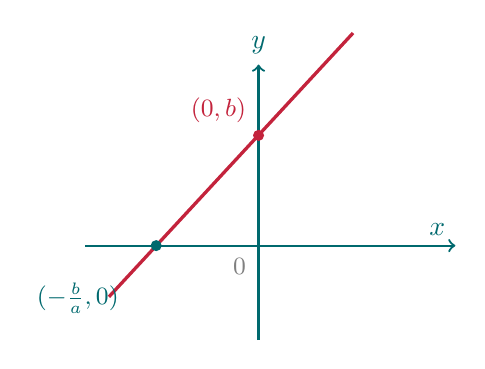
\begin{tikzpicture}[scale=1]
      \draw[->, thick, koreaDarkTeal] (-2.2,0) -- (2.5,0) node[above left, font=\bfseries] {$x$};
      \draw[->, thick, koreaDarkTeal] (0,-1.2) -- (0,2.3) node[above, font=\bfseries] {$y$};
      \node[below left=1pt, font=\fontsize{9}{5}\selectfont, color=gray] at (0,0) {$0$};
      \coordinate (A) at (0, 1.4);
      \coordinate (B) at (-1.3, 0);
      \draw[very thick, color=brandCrimson] (-1.9,-0.65) -- (1.2, 2.7);
      \fill[brandCrimson] (A) circle (2pt) node[above left=1pt, font=\fontsize{9}{5}\selectfont] {$(0,b)$};
      \fill[brandNavy] (B) circle (2pt) node[below left=10pt, font=\fontsize{9}{5}\selectfont] {$(-\frac{b}{a},0)$};
    \end{tikzpicture}
  \end{minipage}
\end{khboxorange}

\vspace{2pt}

\noindent
\exhead{1} \textbf{ចូរសង់សមីការបន្ទាត់នីមួយៗខាងក្រោម ៖}
\begin{center}
\renewcommand{\arraystretch}{1.25}
\begin{tabular}{p{4.4cm}p{4.4cm}p{4.4cm}p{4.4cm}}
  \khlabel{ក} $y = 2x - 5$ & \khlabel{ខ} $y = \frac{1}{2}x - 3$ & \khlabel{គ} $y = 3x$ & \khlabel{ឃ} $y = -\frac{x}{2}$ \\
  \khlabel{ង} $y = 3$ & \khlabel{ច} $y = -\frac{x}{3} + 2$ & \khlabel{ឆ} $y = 3x + 6$ & \khlabel{ជ} $y = 4x - 1$ \\
  \khlabel{ឈ} $y = \frac{2}{3}x - \frac{1}{4}$ & \khlabel{ញ} $y = -\frac{2x}{3}$ & \khlabel{ដ} $y = -6$ & \khlabel{ឋ} $y = -4x$
\end{tabular}
\end{center}

\vspace{2pt}

\begin{khboxorange}
  \begin{itemize}[leftmargin=12pt, itemsep=2.5pt, topsep=1pt, parsep=0pt]
    \item[\color{brandNavy}\ding{228}] \textbf{បន្ទាត់ឈរ ៖} \ \koreahl{$x = h$} \ ស្របនឹងអ័ក្ស $y'y$ កាត់អ័ក្ស $x'x$ ត្រង់ $(h, 0)$ (គ្រប់ចំណុចមាន $x=h$ ថេរ) គ្មានមេគុណប្រាប់ទិស ។
    \item[\color{brandCrimson}\ding{228}] \textbf{បន្ទាត់ដេក ៖} \ \koreahl{$y = k$} \ ស្របនឹងអ័ក្ស $x'x$ កាត់អ័ក្ស $y'y$ ត្រង់ $(0, k)$ (គ្រប់ចំណុចមាន $y=k$ ថេរ) មានមេគុណប្រាប់ទិស $a = 0$ ។
  \end{itemize}
\end{khboxorange}

\vspace{2pt}

\begin{multicols}{2}
  \noindent
  \exhead{2} ចូរសង់បន្ទាត់ដែលមានសមីការ $y = 3$, $x = -1$ និង $y = 2x$ រួចគណនាផ្ទៃក្រឡាខណ្ឌដោយបន្ទាត់ទាំងបីនេះ ។
  \begin{center}
    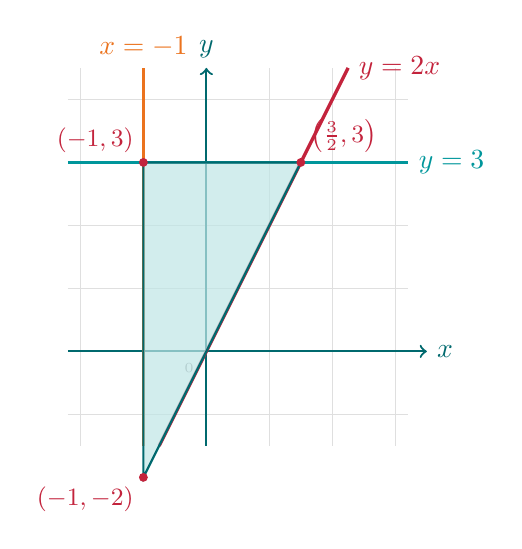
\begin{tikzpicture}[scale=0.8]
      \draw[very thin, gray!25, step=1] (-2.2,-1.5) grid (3.2,4.5);
      \draw[->, thick, koreaDarkTeal] (-2.2,0) -- (3.5,0) node[right, font=\bfseries] {$x$};
      \draw[->, thick, koreaDarkTeal] (0,-1.5) -- (0,4.5) node[above, font=\bfseries] {$y$};
      \node[below left=1pt, font=\tiny, color=gray!80] at (0,0) {$0$};
      
      % Lines
      \draw[very thick, color=brandBlue] (-2.2,3) -- (3.2,3) node[right, font=\kml] {$y = 3$};
      \draw[very thick, color=koreaOrange] (-1,-1.5) -- (-1,4.5) node[above, font=\kml] {$x = -1$};
      \draw[very thick, color=brandCrimson] (-0.75,-1.5) -- (2.25,4.5) node[right, font=\kml] {$y = 2x$};
      
      % Shaded triangle area
      \fill[brandTeal!25, opacity=0.7] (-1,3) -- (1.5,3) -- (-1,-2) -- cycle;
      \draw[thick, brandNavy] (-1,3) -- (1.5,3) -- (-1,-2) -- cycle;
      \fill[brandCrimson] (-1,3) circle (2pt) node[above left, font=\fontsize{9}{6}\selectfont] {$(-1, 3)$};
      \fill[brandCrimson] (1.5,3) circle (2pt) node[above right, font=\fontsize{9}{6}\selectfont] {$\left(\frac{3}{2}, 3\right)$};
      \fill[brandCrimson] (-1,-2) circle (2pt) node[below left, font=\fontsize{9}{6}\selectfont] {$(-1, -2)$};
    \end{tikzpicture}
  \end{center}

  \columnbreak

  \noindent
  \exhead{3} ចូរសង់បន្ទាត់ $y = \frac{x}{2} + 1$ និង $y = -\frac{2x}{3} + 3$ ក្នុងប្លង់កូអរដោនេតែមួយ ។
  \begin{center}
    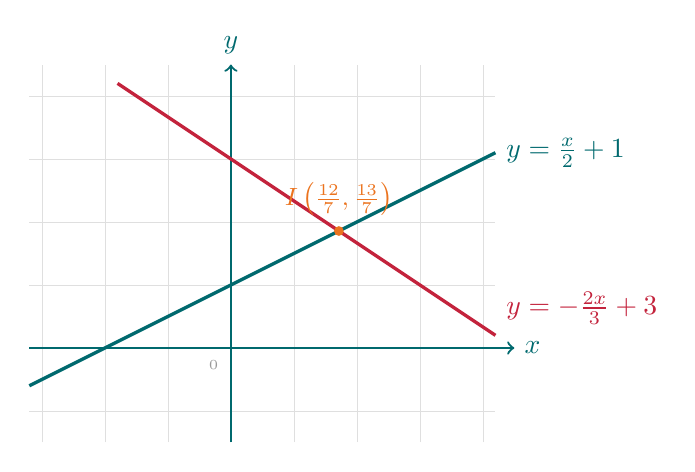
\begin{tikzpicture}[scale=0.8]
      \draw[very thin, gray!25, step=1] (-3.2,-1.5) grid (4.2,4.5);
      \draw[->, thick, koreaDarkTeal] (-3.2,0) -- (4.5,0) node[right, font=\bfseries] {$x$};
      \draw[->, thick, koreaDarkTeal] (0,-1.5) -- (0,4.5) node[above, font=\bfseries] {$y$};
      \node[below left=1pt, font=\tiny, color=gray!80] at (0,0) {$0$};
      
      \draw[very thick, color=brandNavy] (-3.2,-0.6) -- (4.2,3.1) node[right, font=\kml] {$y = \frac{x}{2} + 1$};
      \draw[very thick, color=brandCrimson] (-1.8,4.2) -- (4.2,0.2) node[above right, font=\kml] {$y = -\frac{2x}{3} + 3$};
      \fill[koreaOrange] (1.714, 1.857) circle (2.2pt) node[above=2pt, font=\fontsize{9}{6}\selectfont] {$I\left(\frac{12}{7}, \frac{13}{7}\right)$};
    \end{tikzpicture}
  \end{center}
\end{multicols}

\vspace{3pt}

\noindent
\exhead{4} ចូរសង់បន្ទាត់ $y = \frac{-x + 4}{2}$ \ , \ $y = 2$ និង $x = 4$ ក្នុងប្លង់កូអរដោនេតែមួយ រួចគណនាផ្ទៃក្រឡានៃត្រីកោណដែលខណ្ឌដោយបន្ទាត់ទាំងបីនេះ ។

\newpage

% =========================================================================
% PAGE 3: ២.១ & ២.២ សមីការបន្ទាត់ និងបន្ទាត់ស្រប
% =========================================================================
\khsection{២}{សមីការនៃបន្ទាត់}

\khsubsection{២.១}{សមីការបន្ទាត់កាត់តាមពីរចំណុច}

\begin{khboxorange}
  \begin{itemize}[leftmargin=12pt, itemsep=2pt, topsep=1pt, parsep=0pt]
    \item[\color{brandNavy}\ding{228}] \textbf{គំនិត  ៖} សមីការបន្ទាត់កើតចេញពីនិយមន័យមេគុណប្រាប់ទិស $a = \frac{y - y_1}{x - x_1}$ ដោយគ្រាន់តែគុណខ្វែង ៖
    \begin{equation*}
      \koreahl{$y - y_1 = a(x - x_1)$} \quad \text{ដែល } \koreahl{$a = \frac{y_2 - y_1}{x_2 - x_1}$} \quad \left(\text{ឬ } \frac{y - y_1}{x - x_1} = \frac{y_2 - y_1}{x_2 - x_1}\right)
    \end{equation*}
  \end{itemize}
\end{khboxorange}

\vspace{1pt}

\noindent
\exhead{1} \textbf{ចូររកសមីការបន្ទាត់ដែលកាត់តាមពីរចំណុចខាងក្រោម ៖}
\begin{center}
\renewcommand{\arraystretch}{1.2}
\begin{tabular}{p{8.8cm}p{8.8cm}}
  \khlabel{ក} $A(0, 0)$ និង $B(5, 2)$ & \khlabel{ខ} $A(-2, 0)$ និង $B(2, -3)$ \\
  \khlabel{គ} $A(-1, 0)$ និង $B(2, -3)$ & \khlabel{ឃ} $A(-2, -1)$ និង $B(-2, -2)$ \\
  \khlabel{ង} $S(3, -2)$ និង $T(5, 4)$ & \khlabel{ច} $M(-3, -1)$ និង $N(-4, 2)$ \\
  \khlabel{ឆ} $A\left(\frac{1}{2}, 2\right)$ និង $B(-3, -1)$ & \khlabel{ជ} $A\left(\frac{2}{3}, 0\right)$ និង $B\left(-2, -\frac{1}{4}\right)$
\end{tabular}
\end{center}

\vspace{1pt}

\noindent
\exhead{2} \textbf{ចូររកសមីការបន្ទាត់កាត់តាមពីរចំណុច} $(-2, 7)$ និង $(2, -1)$ ។

\vspace{3pt}

\khsubsection{២.២}{លក្ខខណ្ឌនៃបន្ទាត់ស្រប}

\begin{khcard}
  \begin{minipage}[c]{0.64\textwidth}
    \textbf{\color{brandNavy}សង់បន្ទាត់ពីរដែលមានមេគុណប្រាប់ទិសស្មើគ្នា ៖}\\
    $d_1 : y = \frac{x}{2} + 1$ \quad និង \quad $d_2 : y = \frac{x}{2} - 1$\\[2pt]
    \centering
    \renewcommand{\arraystretch}{1.05}
    \begin{tabular}{|c|c|c|}
      \hline
      \rowcolor{brandTeal!15}
      \multicolumn{3}{|c|}{\textbf{តារាងតម្លៃលេខ } $d_1$} \\
      \hline
      $x$ & $0$ & $-2$ \\
      \hline
      $y$ & $1$ & $0$ \\
      \hline
    \end{tabular}
    \qquad
    \begin{tabular}{|c|c|c|}
      \hline
      \rowcolor{brandCrimson!15}
      \multicolumn{3}{|c|}{\textbf{តារាងតម្លៃលេខ } $d_2$} \\
      \hline
      $x$ & $0$ & $2$ \\
      \hline
      $y$ & $-1$ & $0$ \\
      \hline
    \end{tabular}
    \\[3pt]
    \raggedright
    \begin{itemize}[leftmargin=12pt, itemsep=1.5pt, topsep=1pt, parsep=0pt]
      \item ដោយមេគុណប្រាប់ទិសនៃបន្ទាត់ទាំងពីរស្មើគ្នា គឺ $a_1 = a_2 = \frac{1}{2}$
      \item \textbf{គំនិត ៖} បន្ទាត់ទាំងពីរមាន\textbf{កម្រិតចោតស្មើគ្នា} មិនអាចកាត់គ្នាឡើយ
      \item គេសង្កេតឃើញថា បន្ទាត់ទាំងពីរ $d_1$ និង $d_2$ គឺជា\textbf{បន្ទាត់ស្របគ្នា} ($d_1 \parallel d_2$) ។
    \end{itemize}
  \end{minipage}\hfill
  \begin{minipage}[c]{0.34\textwidth}
    \centering
    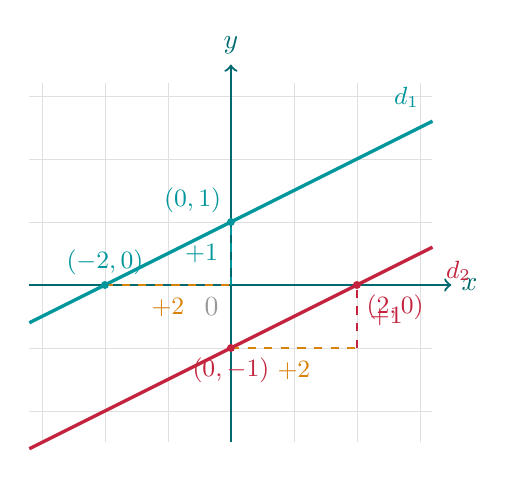
\begin{tikzpicture}[scale=0.8]
      \draw[very thin, gray!25, step=1] (-3.2,-2.5) grid (3.2,3.2);
      \draw[->, thick, koreaDarkTeal] (-3.2,0) -- (3.5,0) node[right, font=\bfseries] {$x$};
      \draw[->, thick, koreaDarkTeal] (0,-2.5) -- (0,3.5) node[above, font=\bfseries] {$y$};
      \node[below left=1pt,  color=gray!80] at (0,0) {$0$};
      
      \draw[very thick, color=brandTeal] (-3.2,-0.6) -- (3.2,2.6) node[above left=1pt, font=\fontsize{9}{6}\selectfont\bfseries, color=brandTeal] {$d_1$};
      \draw[very thick, color=brandCrimson] (-3.2,-2.6) -- (3.2,0.6) node[below right=1pt, font=\fontsize{9}{6}\selectfont\bfseries, color=brandCrimson] {$d_2$};
      
      % Slope steps for d1
      \draw[thick, dashed, color=brandGold] (-2,0) -- (0,0) node[midway, below=1pt, font=\fontsize{9}{4.5}\selectfont\bfseries, color=brandGold] {$+2$};
      \draw[thick, dashed, color=brandTeal] (0,0) -- (0,1) node[midway, left=1pt, font=\fontsize{9}{4.5}\selectfont\bfseries, color=brandTeal] {$+1$};
      
      % Slope steps for d2
      \draw[thick, dashed, color=brandGold] (0,-1) -- (2,-1) node[midway, below=1pt, font=\fontsize{9}{4.5}\selectfont\bfseries, color=brandGold] {$+2$};
      \draw[thick, dashed, color=brandCrimson] (2,-1) -- (2,0) node[midway, right=1pt, font=\fontsize{9}{4.5}\selectfont\bfseries, color=brandCrimson] {$+1$};
      
      \fill[brandTeal] (0,1) circle (1.8pt) node[above left, font=\fontsize{9}{5}\selectfont] {$(0,1)$};
      \fill[brandTeal] (-2,0) circle (1.8pt) node[above, font=\fontsize{9}{5}\selectfont] {$(-2,0)$};
      \fill[brandCrimson] (0,-1) circle (1.8pt) node[below , font=\fontsize{9}{5}\selectfont] {$(0,-1)$};
      \fill[brandCrimson] (2,0) circle (1.8pt) node[below right, font=\fontsize{9}{5}\selectfont] {$(2,0)$};
    \end{tikzpicture}
  \end{minipage}
\end{khcard}

\vspace{2pt}

\begin{khboxorange}[top=4pt, bottom=4pt]
  \begin{itemize}[leftmargin=12pt, itemsep=2pt, topsep=1pt, parsep=0pt]
    \item[\color{brandNavy}\ding{228}] \textbf{ទ្រឹស្ដីបទបន្ទាត់ស្រប ៖} បន្ទាត់ពីរ $d_1 : y = ax + b$ និង $d_2 : y = a'x + b'$ ស្របគ្នា លុះត្រាតែមាន\textbf{កម្រិតចោតស្មើគ្នា} ($a = a'$) និងចំណុចចាប់ផ្ដើមខុសគ្នា ៖
    \begin{equation*}
      \koreahl{$d_1 \parallel d_2 \iff a = a' \quad \text{និង } b \neq b'$}
    \end{equation*}
    \item[\color{brandCrimson}\ding{228}] \textbf{សម្គាល់ ៖} បើ $a = a'$ និង $b = b'$ នោះបន្ទាត់ទាំងពីរត្រួតស៊ីគ្នា ($d_1 \equiv d_2$) ។
  \end{itemize}
\end{khboxorange}

\vspace{2pt}

\noindent
\exhead{3} ចូរសង់បន្ទាត់ $d : y = \frac{3}{2}x - 3$ និងដៅចំណុច $A(-1, 1)$ និង $B(1, 4)$ ។ ចូរបញ្ជាក់ថា $d \parallel AB$ ។\\[2pt]
\exhead{4} គេឱ្យបួនចំណុច $A(-1, 0), B(0, 2), C(3, 2)$ និង $D(4, 4)$ ។ ចូរគណនាមេគុណប្រាប់ទិសនៃបន្ទាត់ $AB$ និង $CD$ ហើយបញ្ជាក់ថាវាជាបន្ទាត់ស្របគ្នា ។\\[2pt]
\exhead{5} \textbf{ចូររកសមីការបន្ទាត់ដែលកាត់តាមមួយចំណុច ហើយស្របនឹងបន្ទាត់មួយ ៖}
\begin{center}
\renewcommand{\arraystretch}{1.2}
\begin{tabular}{p{8.8cm}p{8.8cm}}
  \khlabel{ក} កាត់តាម $A(2, 0)$ ស្របនឹងបន្ទាត់ $y = 2x + 4$ & \khlabel{ខ} កាត់តាម $A(2, 5)$ ស្របនឹងបន្ទាត់ $y = 3x + 4$ \\
  \khlabel{គ} កាត់តាម $A(0, 0)$ ស្របនឹងបន្ទាត់ $y = 3x - 1$ & \khlabel{ឃ} កាត់តាម $A(2, 0)$ ស្របនឹងបន្ទាត់ $y = -x + 4$ \\
  \khlabel{ង} កាត់តាម $A(2, 2)$ ស្របនឹងបន្ទាត់ $2x + y = 4$ & \khlabel{ច} កាត់តាម $A(6, 3)$ ស្របនឹងបន្ទាត់ $x - 3y = 9$ \\
  \khlabel{ឆ} កាត់តាម $A(-2, -3)$ ស្របនឹងបន្ទាត់ $3x + y = -2$ & \khlabel{ជ} កាត់តាម $A(-4, 2)$ ស្របនឹងបន្ទាត់ $\frac{1}{2}x + y - 2 = 0$
\end{tabular}
\end{center}

\newpage

% =========================================================================
% PAGE 4: ២.៣ បន្ទាត់កែង & ផ្នែកទី ៣ ៖ អនុវត្តន៍
% =========================================================================
\khsubsection{២.៣}{លក្ខខណ្ឌនៃបន្ទាត់កែង}

\begin{khboxorange}[top=2pt, bottom=2pt, left=6pt, right=6pt]
  \begin{minipage}[c]{0.77\textwidth}
    \textbf{\color{brandNavy}\ding{228}\ ទ្រឹស្ដីបទបន្ទាត់កែង ៖} បន្ទាត់ពីរ $d_1 : y = ax + b$ និង $d_2 : y = a'x + b'$ កែងគ្នាលុះត្រាតែមេគុណប្រាប់ទិសជា\textbf{ចំនួនច្រាសនិងផ្ទុយសញ្ញាគ្នា} ៖\\[2pt]
    \centerline{\koreahl{$d_1 \perp d_2 \iff a \times a' = -1 \quad \left(\text{ឬ } a' = -\frac{1}{a}\right)$}}
  \end{minipage}\hfill
  \begin{minipage}[c]{0.21\textwidth}
    \centering
    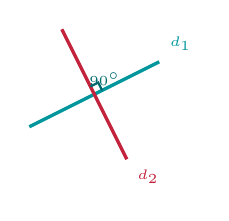
\begin{tikzpicture}[scale=0.55]
      \draw[very thick, color=brandTeal] (-1.5,-0.75) -- (1.5,0.75) node[above right, font=\tiny\kml] {$d_1$};
      \draw[very thick, color=brandCrimson] (-0.75,1.5) -- (0.75,-1.5) node[below right, font=\tiny\kml] {$d_2$};
      \draw[thick, brandNavy] (0.18,0.09) -- (0.09,0.27) -- (-0.09,0.18);
      \node[font=\fontsize{5}{5}\selectfont\bfseries, color=brandNavy] at (0.24, 0.35) {$90^\circ$};
    \end{tikzpicture}
  \end{minipage}
\end{khboxorange}

\vspace{0.5pt}

\noindent
\begin{minipage}[t]{0.49\textwidth}\raggedright
  \exhead{1} រកតម្លៃ $a$ ដើម្បីឱ្យបន្ទាត់ $y = ax + 3$ និង $y - 2x = 1$ កែងគ្នា ។
\end{minipage}\hfill
\begin{minipage}[t]{0.49\textwidth}\raggedright
  \exhead{2} រកសមីការបន្ទាត់កាត់តាម $A(-1, 2)$ ហើយកែងនឹងបន្ទាត់ $y = 3x$ ។
\end{minipage}

\vspace{0.5pt}

\noindent
\exhead{3} គេឱ្យបីចំណុច $A(0, 3), B(2, 0)$ និង $C\left(4, \frac{17}{3}\right)$ ។ ចូរបញ្ជាក់ថា $AB \perp AC$ ។\\[1pt]
\exhead{4} \textbf{ចូររកសមីការបន្ទាត់ដែលកាត់តាមមួយចំណុច ហើយកែងនឹងបន្ទាត់មួយទៀត ៖}\\[1pt]
\noindent
\setlength{\tabcolsep}{3pt}
\renewcommand{\arraystretch}{0.95}
\begin{tabular}{p{4.6cm}p{4.6cm}p{4.6cm}p{4.6cm}}
  \khlabel{ក} កាត់ $A(0, 0)$ កែង$y = 2x + 1$ & \khlabel{ខ} កាត់ $A(2, 2)$ កែង $y = 2x + 4$ & \khlabel{គ} $A(1, 2)$ កែង $y = -x - 1$ & \khlabel{ឃ} $A(-2, 0)$ កែង $y = 3x + 4$ 
\end{tabular}

\vspace{0.5pt}

\noindent
\exhead{5} \textbf{ចូររកសមីការបន្ទាត់ដែលកាត់តាមមួយចំណុច ហើយកែងនឹងបន្ទាត់មួយទៀត ៖}\\[1pt]
\khlabel{ក} កាត់តាម $A(2, -1)$ កែង $2y - x - 1 = 0$ ។ \qquad
\khlabel{ខ} កាត់តាម $A\left(-\frac{1}{2}, 0\right)$កែង $y = 2x$ ។

\vspace{0.5pt}

% =========================================================================
% ផ្នែកទី ៣ ៖ អនុវត្តន៍
% =========================================================================
\khsection{៣}{អនុវត្តន៍}

\begin{khcard}[top=2pt, bottom=2pt]
  \exhead{6} ថាសចម្រៀងដ៏ល្បីមួយបានផ្ដើមលក់នៅខែមករា បន្ទាប់ពីបានលក់ច្រើនខែនៅខែមករានោះមក ថាសនេះនៅតែលក់បានជាបន្តបន្ទាប់ទៅតាមខែនីមួយៗ ដោយអត្រា $500$ ថាសក្នុងមួយខែរហូតដល់ដំណាច់ឆ្នាំ នាឆ្នាំដដែល គេសរុបឃើញលក់បាន $9700$ ថាស ។
  \begin{itemize}[leftmargin=17pt, itemsep=0.2pt, topsep=0.5pt, parsep=0pt]
    \item[\khlabel{ក}] ចូរសរសេរសមីការដែលតាងឱ្យការលក់ថាសតាមខែនីមួយៗ ។
    \item[\khlabel{ខ}] ចូររកចំនួនថាសដែលបានលក់នៅខែមករា ។
    \item[\khlabel{គ}] គិតត្រឹមខែសីហា គេលក់ជាក់ស្ដែងបាន $7600$ ថាស ។ តើចំនួនលក់ជាក់ស្ដែងមានលំអៀងជាមួយចំនួនគណនាតាមសមីការប៉ុន្មាន ?
  \end{itemize}
  \vspace{1pt}
  \begin{tcolorbox}[enhanced, colback=koreaBeige, colframe=brandNavy!40, boxrule=0.6pt, arc=3pt, left=10pt, right=5pt, top=2.5pt, bottom=2.5pt, drop fuzzy shadow=brandNavy!10]
    \begin{minipage}[c]{0.58\textwidth}
      \textbf{\color{brandNavy}\ding{72}\ ដំណោះស្រាយលម្អិត៖}\\[1.5pt]
      \textbf{\color{brandCrimson}\ding{228} គំរូ ៖} តាង $x$ ជាខែ ($x=1,\dots,12$), $y$ ជាចំនួនថាសសរុប ។ អត្រាលក់ថេរ $500$ ថាស/ខែ ($a=500$) នាំឱ្យសមីការមានរាង \ $y = 500x + b$ ។
      \begin{itemize}[leftmargin=10pt, itemsep=0.6pt, topsep=0.5pt, parsep=0pt]
        \item[\khlabel{ក}] \textbf{សមីការតាងការលក់ ៖} ដំណាច់ឆ្នាំ ($x=12$) លក់បាន $y=9700$ ថាស ៖\\
          $9700 = 500(12) + b \iff 9700 = 6000 + b \implies b = 3700$ ។\\
          \textbf{ដូចនេះ ៖} សមីការតាងការលក់គឺ \ \koreahl{$y = 500x + 3700$} ។
        \item[\khlabel{ខ}] \textbf{ចំនួនថាសលក់នៅខែមករា ($x=1$) ៖}\\
          $y = 500(1) + 3700 = 500 + 3700 = \mathbf{4200\text{ ថាស}}$ ។
        \item[\khlabel{គ}] \textbf{គណនាតម្លៃលំអៀងត្រឹមខែសីហា ($x=8$) ៖}\\
          • តាមសមីការ ៖ $y = 500(8) + 3700 = 7700\text{ ថាស}$ ។\\
          • ជាក់ស្ដែង ៖ $7600\text{ ថាស} \longrightarrow \text{លំអៀង} = 7700 - 7600 = \mathbf{100\text{ ថាស}}$ ។
      \end{itemize}
    \end{minipage}\hfill%
    \begin{minipage}[c]{0.40\textwidth}
      \centering
      \begin{tikzpicture}[x=0.33cm, y=0.00021cm]
        % Axes
        \draw[->, >=stealth, thick, koreaDarkTeal] (0,2000) -- (13.2,2000) node[right=1pt, font=\fontsize{9}{6}\selectfont\bfseries, text=koreaDarkTeal] {$x$ (ខែ)};
        \draw[->, >=stealth, thick, koreaDarkTeal] (0,2000) -- (0,13700) node[above=1pt, font=\fontsize{9}{6}\selectfont\bfseries, text=koreaDarkTeal] {$y$ (ថាស)};
        
        % Axis break mark on y-axis
        \draw[thick, koreaDarkTeal] (-0.15, 2300) -- (0.15, 2500);
        \draw[thick, koreaDarkTeal] (-0.15, 2450) -- (0.15, 2650);
        
        % Projections (Grid lines)
        \draw[densely dashed, gray!45, line width=0.4pt] (1,2000) -- (1,4200) -- (0,4200);
        \draw[densely dashed, gray!45, line width=0.4pt] (8,2000) -- (8,7700) -- (0,7700);
        \draw[densely dashed, gray!45, line width=0.4pt] (12,2000) -- (12,9700) -- (0,9700);
        
        % Slope Step Triangle (from x=2 to x=4)
        \fill[brandGold!18] (2,4700) -- (4,4700) -- (4,5700) -- cycle;
        \draw[->, >=stealth, thick, color=brandGold] (2,4700) -- (4,4700) node[midway, below=0.5pt, font=\fontsize{5}{5}\selectfont\bfseries, text=brandGold] {$\Delta x = 2$};
        \draw[->, >=stealth, thick, color=brandCrimson] (4,4700) -- (4,5700) node[midway, right=0.5pt, font=\fontsize{5}{5}\selectfont\bfseries, text=brandCrimson] {$\Delta y = 1000$};
        \node[font=\fontsize{4.8}{4.8}\selectfont\bfseries, text=brandCrimson] at (3.1,6250) {$a = 500$};
        
        % Line
        \draw[very thick, brandCrimson] (0,3700) -- (12.4,9900);
        \node[above=1.5pt, sloped, font=\fontsize{5.2}{5.2}\selectfont\bfseries, text=brandCrimson] at (10.2,8800) {$y=500x+3700$};
        
        % Points & Coordinates
        \fill[brandNavy] (0,3700) circle (1.5pt) node[left=1.5pt, font=\fontsize{5}{5}\selectfont\bfseries, text=brandNavy] {$3700$};
        \fill[brandNavy] (1,4200) circle (1.5pt) node[above left=0.5pt, font=\fontsize{5}{5}\selectfont\bfseries, text=brandNavy] {$(1,4200)$};
        
        % August Points & Error
        \fill[brandCrimson] (8,7700) circle (1.6pt) node[above left=0.5pt, font=\fontsize{4.8}{4.8}\selectfont\bfseries, text=brandCrimson] {សមីការ $(8,7700)$};
        \fill[koreaOrange] (8,7600) circle (1.6pt) node[below right=0.5pt, font=\fontsize{4.8}{4.8}\selectfont\bfseries, text=koreaOrange] {ជាក់ស្ដែង $(8,7600)$};
        \draw[<->, >=stealth, very thick, color=brandGold] (8.2,7600) -- (8.2,7700) node[midway, right=0.5pt, font=\fontsize{5}{5}\selectfont\bfseries, text=brandGold] {$\Delta = 100$};
        
        % Year-End Point
        \fill[brandNavy] (12,9700) circle (1.6pt) node[below right=0.5pt, font=\fontsize{4.8}{4.8}\selectfont\bfseries, text=brandNavy] {ដំណាច់ឆ្នាំ $(12,9700)$};
        
        % Axis Ticks
        \draw[koreaDarkTeal, line width=0.4pt] (1,1900) -- (1,2100);
        \draw[koreaDarkTeal, line width=0.4pt] (8,1900) -- (8,2100);
        \draw[koreaDarkTeal, line width=0.4pt] (12,1900) -- (12,2100);
        \node[below=1pt, font=\fontsize{5.5}{5.5}\selectfont\bfseries] at (1,1950) {$1$};
        \node[below=1pt, font=\fontsize{5.5}{5.5}\selectfont\bfseries] at (8,1950) {$8$};
        \node[below=1pt, font=\fontsize{5.5}{5.5}\selectfont\bfseries] at (12,1950) {$12$};
      \end{tikzpicture}
    \end{minipage}
  \end{tcolorbox}
\end{khcard}

\vspace{0.5pt}

\begin{khcard}[top=1.5pt, bottom=1.5pt]
  \exhead{7} ការរីកចម្រើននៃផ្នែកឧស្សាហកម្ម និងសេវាកម្មនានាបានបណ្ដាលឱ្យចំនួនកសិករថយចុះជាលំដាប់ទៅតាមអត្រា $0.8\%$ ក្នុងមួយឆ្នាំ ។ បើកសិករមានចំនួន $80\%$ នៅឆ្នាំ $2000$ ៖\\[1pt]
  \khlabel{ក} រកសមីការដែលទាក់ទងទៅនឹងភាគរយនៃកសិករដែលបានថយចុះទៅតាមឆ្នាំ $x$ ។ \qquad
  \khlabel{ខ} ប៉ាន់ស្មានរកចំនួនភាគរយនៃកសិករនៅឆ្នាំ $2008$ ។\\[1.2pt]
  \colorbox{koreaYellow!45}{\fontsize{7.5}{7.5}\selectfont\textbf{\color{brandGold}\ding{72}\ Hint ៖} តាង $x$ ជាចំនួនឆ្នាំគិតពីឆ្នាំ $2000$ ($x=0$) $\Rightarrow a = -0.8$ និង $b = 80 \longrightarrow y = -0.8x + 80$ ។ ឆ្នាំ $2008$ ត្រូវនឹង $x = 8$ ។}
\end{khcard}

\vspace{0.5pt}

\begin{khcard}[top=1.5pt, bottom=1.5pt]
  \exhead{8} នៅម៉ោង $12$ ថ្ងៃត្រង់កម្ដៅមានសីតុណ្ហភាព $40^\circ\text{C}$ ។ សីតុណ្ហភាពនេះនឹងថយចុះវិញក្នុងអត្រា $2^\circ\text{C}$ ក្នុងមួយម៉ោង ។ តើនៅម៉ោងប៉ុន្មានទើបមានសីតុណ្ហភាពស្មើនឹង $26^\circ\text{C}$ ?\\[1.2pt]
  \colorbox{koreaYellow!45}{\fontsize{7.5}{7.5}\selectfont\textbf{\color{brandGold}\ding{72}\ Hint ៖} តាង $x$ ជាចំនួនម៉ោងគិតពីម៉ោង $12$ ថ្ងៃត្រង់ ($x=0$) នាំឱ្យ $T = -2x + 40$ ។ ជំនួស $T = 26 \Rightarrow x = 7$ ម៉ោង (គឺម៉ោង $7$ យប់) ។}
\end{khcard}

\newpage

% =========================================================================
% PAGE 5: ផ្នែកទី ៤ ៖ លំហាត់អនុវត្តន៍បន្ថែម (លំហាត់ ០១ ដល់ ១៥)
% =========================================================================
\khsection{៤}{លំហាត់អនុវត្តន៍បន្ថែម}

\begin{multicols}{2}
\raggedright

  % Problem 1
  \noindent
  \begin{minipage}{\linewidth}\raggedright
    \exhead{1} \textbf{ចូររកមេគុណប្រាប់ទិសនៃបន្ទាត់ដែលកាត់តាមពីរចំណុច ៖}\\[2pt]
    \begin{tabular}{@{}p{0.48\linewidth}@{\hspace{6pt}}p{0.48\linewidth}@{}}
      \khlabel{ក} $(3, 1)$ និង $(5, 4)$ & \khlabel{ខ} $(3, 0)$ និង $(-3, -6)$ \\[3pt]
      \khlabel{គ} $(-2, -1)$ និង $(-4, -4)$ & \khlabel{ឃ} $(1, 4)$ និង $(4, -2)$
    \end{tabular}
  \end{minipage}

  \vspace{5pt}

  % Problem 2
  \noindent
  \begin{minipage}{\linewidth}\raggedright
    \exhead{2} \textbf{ចូរសរសេរសមីការនៃបន្ទាត់ដែលកាត់តាមពីរចំណុច ៖}\\[2pt]
    \begin{tabular}{@{}p{0.48\linewidth}@{\hspace{6pt}}p{0.48\linewidth}@{}}
      \khlabel{ក} $(-6, 1)$ និង $(6, -2)$ & \khlabel{ខ} $(3, -4)$ និង $(-9, 2)$ \\[3pt]
      \khlabel{គ} $(2, 0)$ និង $(1, -8)$ & \khlabel{ឃ} $(-4.2, -4)$ និង $(-2.2, 6)$ \\[3pt]
      \khlabel{ង} $(2.5, -1)$ និង $(0.5, 1)$ & \khlabel{ច} $(0, 5)$ និង $(3, -2.5)$
    \end{tabular}
  \end{minipage}

  \vspace{5pt}

  % Problem 3
  \noindent
  \begin{minipage}{\linewidth}\raggedright
    \exhead{3} ការយល់ដឹងពីគ្រោះថ្នាក់នៃបារី បណ្ដាលឱ្យចំនួនអ្នកជក់បានថយចុះចាប់ពីឆ្នាំ $1992$ មក ។ បើអ្នកជក់មានចំនួន $38\%$ នៅឆ្នាំ $1992$ ហើយចំនួននេះបានថយចុះមកត្រឹម $15.5\%$ នៅឆ្នាំ $2007$ ។ ចូររកសមីការដែលទាក់ទងនឹងចំនួនអ្នកជក់ និងចំនួនឆ្នាំ ។
  \end{minipage}

  \vspace{5pt}

  % Problem 4
  \noindent
  \begin{minipage}{\linewidth}\raggedright
    \exhead{4} ចូរសរសេរសមីការ និងសង់បន្ទាត់ដែលមានមេគុណប្រាប់ទិស $m$ ហើយកាត់តាមចំណុច $P$ រួចរកកូអរដោនេនៃចំណុចប្រសព្វរវាងបន្ទាត់ និងអ័ក្ស ៖\\[2pt]
    \begin{tabular}{@{}p{0.48\linewidth}@{\hspace{6pt}}p{0.48\linewidth}@{}}
      \khlabel{ក} $m = 1$ និង $P(0, 2)$ & \khlabel{ខ} $m = -1$ និង $P(1, 0)$ \\[3pt]
      \khlabel{គ} $m = -2$ និង $P(3, -1)$ & \khlabel{ឃ} $m = \frac{3}{5}$ និង $P(-1, -4)$ \\[3pt]
      \khlabel{ង} $m = 0$ និង $P(2, 1)$ & \khlabel{ច} $m = -\frac{3}{2}$ និង $P(0, 3)$
    \end{tabular}
  \end{minipage}

  \vspace{5pt}

  % Problem 5
  \noindent
  \begin{minipage}{\linewidth}\raggedright
    \exhead{5} ក្នុងចំណោមបន្ទាត់ទាំងបីខាងក្រោម តើមួយណាស្របគ្នា ?\\[2pt]
    \begin{tabular}{@{}p{0.48\linewidth}@{\hspace{6pt}}p{0.48\linewidth}@{}}
      \khlabel{ក} $2x + 3y = -11$ & \khlabel{ខ} $4x + 8y - 1 = 0$ \\[3pt]
      \multicolumn{2}{@{}l@{}}{\khlabel{គ} $y = -\frac{2}{3}x + 1$}
    \end{tabular}
  \end{minipage}

  \vspace{5pt}

  % Problem 6
  \noindent
  \begin{minipage}{\linewidth}\raggedright
    \exhead{6} ចូររកមេគុណប្រាប់ទិសនៃបន្ទាត់តាងសមីការខាងក្រោម រួចប្រាប់ថាតើគូសមីការណាដែលមានបន្ទាត់ស្របគ្នា ៖\\[2pt]
    \begin{tabular}{@{}l@{\hspace{5pt}}l@{\hspace{6pt}}l@{\hspace{6pt}}l@{}}
      \khlabel{ក} & $y = x + 4$ & និង & $x - y + 5 = 0$ \\[2pt]
      \khlabel{ខ} & $y = 2x - 3$ & និង & $x + 2y + 1 = 0$ \\[2pt]
      \khlabel{គ} & $3x - y + 4 = 0$ & និង & $y - 2 = 3(x + 1)$ \\[2pt]
      \khlabel{ឃ} & $2y = 5x + 6$ & និង & $5x + 2y - 1 = 0$
    \end{tabular}
  \end{minipage}

  \vspace{5pt}

  % Problem 7
  \noindent
  \begin{minipage}{\linewidth}\raggedright
    \exhead{7} តើគូសមីការណាខ្លះដែលមានបន្ទាត់កែងគ្នា ?\\[2pt]
    \begin{tabular}{@{}l@{\hspace{5pt}}l@{\hspace{6pt}}l@{\hspace{6pt}}l@{}}
      \khlabel{ក} & $y = 3x + 1$ & និង & $y = -\frac{1}{3}x$ \\[2pt]
      \khlabel{ខ} & $y = 2x + 5$ & និង & $x - 2y + 6 = 0$ \\[2pt]
      \khlabel{គ} & $y = 5x - 4$ & និង & $x + 5y - 1 = 0$ \\[2pt]
      \khlabel{ឃ} & $-2x + y = -2$ & និង & $3(x + y) - 2 = 0$
    \end{tabular}
  \end{minipage}

  \vspace{5pt}

  % Problem 8
  \noindent
  \begin{minipage}{\linewidth}\raggedright
    \exhead{8} ចូររកសមីការបន្ទាត់ដែលស្របនឹង ៖\\[2pt]
    \begin{tabular}{@{}l@{\hspace{5pt}}l@{\hspace{6pt}}l@{}}
      \khlabel{ក} & $y = 3x - 4$ & ហើយកាត់តាមចំណុច $(5, 1)$ \\[2pt]
      \khlabel{ខ} & $3x - 2y + 5 = 0$ & ហើយកាត់តាមចំណុច $(-2, 4)$ \\[2pt]
      \khlabel{គ} & $2x + 2y + 9 = 0$ & ហើយកាត់តាមចំណុច $\left(-\frac{5}{3}, 0\right)$ \\[2pt]
      \khlabel{ឃ} & $x - 5y + 6 = 0$ & ហើយកាត់តាមចំណុច $(0, 0)$
    \end{tabular}
  \end{minipage}

  \vspace{5pt}

  % Problem 9
  \noindent
  \begin{minipage}{\linewidth}\raggedright
    \exhead{9} ចូរកំណត់សមីការបន្ទាត់ដែលកែងនឹង ៖\\[2pt]
    \begin{tabular}{@{}l@{\hspace{5pt}}l@{\hspace{6pt}}l@{}}
      \khlabel{ក} & $y = \frac{1}{2}x + 4$ & ហើយកាត់តាមចំណុច $(5, 0)$ \\[2pt]
      \khlabel{ខ} & $x - y + 5 = 0$ & ហើយកាត់តាមចំណុច $(0, 0)$ \\[2pt]
      \khlabel{គ} & $8x + 3y + 1 = 0$ & ហើយកាត់តាមចំណុច $(-1, 4)$ \\[2pt]
      \khlabel{ឃ} & $y = -x + 6$ & ហើយកាត់តាមចំណុច $\left(-4, -\frac{2}{3}\right)$
    \end{tabular}
  \end{minipage}

  \vspace{5pt}

  % Problem 10
  \noindent
  \begin{minipage}{\linewidth}\raggedright
    \exhead{10} \textbf{គេមានបន្ទាត់ និងចំណុចក្នុងប្លង់ ៖}\\[2pt]
    \begin{itemize}[leftmargin=16pt, itemsep=2pt, topsep=1pt, parsep=0pt]
      \item[\khlabel{ក}] ចូរកំណត់សមីការនៃបន្ទាត់ $d_1$ កាត់តាមចំណុច $A(-3, 5)$ ដែលមានមេគុណប្រាប់ទិសស្មើនឹង $-2$ រួចសង់បន្ទាត់នេះ ។
      \item[\khlabel{ខ}] គេមានសមីការបន្ទាត់ $d_2 : y = (m - 1)x + 2$ ។ ចូរកំណត់តម្លៃ $m$ ដើម្បីឱ្យបន្ទាត់ $d_2$ ស្រប $d_1$ ។ តើមានតម្លៃ $m$ ដែលឱ្យ $d_2$ កែងនឹង $d_1$ ដែរឬទេ ? ចូរសរសេរសមីការនៃបន្ទាត់ត្រូវនឹងតម្លៃ $m$ នីមួយៗ រួចសង់បន្ទាត់ទាំងនោះ ។
      \item[\khlabel{គ}] $B$ ជាចំណុចដែលមានកូអរដោនេ $(6, 0)$ ។ ចូរសរសេរសមីការនៃបន្ទាត់កាត់តាម $A$ និង $B$ រួចបញ្ជាក់ចំណុចកាត់នឹងអ័ក្ស $y'y$ ។
    \end{itemize}
  \end{minipage}

  \vspace{5pt}

  % Problem 11
  \noindent
  \begin{minipage}{\linewidth}\raggedright
    \exhead{11} ក្នុងតម្រុយអរតូណរមេ គេឱ្យបីចំណុច $A(0, 6)$, $B(-3, 0)$ និង $C(6, 0)$ ៖\\[2pt]
    \begin{itemize}[leftmargin=16pt, itemsep=2pt, topsep=1pt, parsep=0pt]
      \item[\khlabel{ក}] ចូររកសមីការនៃបន្ទាត់ $AB$ និង $AC$ ។
      \item[\khlabel{ខ}] ចូររកសមីការនៃបន្ទាត់ $D$ កាត់តាមចំណុច $C$ ហើយកែងនឹងបន្ទាត់ $AB$ ។
      \item[\khlabel{គ}] ចូររកសមីការនៃបន្ទាត់ $D'$ កាត់តាមចំណុច $B$ ហើយស្របនឹងបន្ទាត់ $AC$ ។
    \end{itemize}
  \end{minipage}

  \vspace{5pt}

  % Problem 12
  \noindent
  \begin{minipage}{\linewidth}\raggedright
    \exhead{12} \textbf{ក្នុងតម្រុយអរតូណរមេ ៖}\\[2pt]
    \begin{itemize}[leftmargin=16pt, itemsep=2pt, topsep=1pt, parsep=0pt]
      \item[\khlabel{ក}] រកសមីការនៃបន្ទាត់កាត់តាមចំណុច $A(6, 2)$ និង $B(2, -2)$ ។ ចូររកសមីការនៃខ្សែមេដ្យាទ័ររបស់ $AB$ ។
      \item[\khlabel{ខ}] គេឱ្យចំណុច $C(-2, 6)$ ។ ចូរបង្ហាញថា $CAB$ ជាត្រីកោណសមបាត ។
      \item[\khlabel{គ}] ចូររកសមីការនៃបន្ទាត់ $C_2$ កាត់តាមចំណុច $C$ ហើយស្របនឹងបន្ទាត់ $AB$ ។
      \item[\khlabel{ឃ}] ចូរបង្ហាញថាបន្ទាត់ $C_2$ កាត់តាម $M(-5, 3)$ ។
    \end{itemize}
  \end{minipage}

  \vspace{5pt}

  % Problem 13
  \noindent
  \begin{minipage}{\linewidth}\raggedright
    \exhead{13} ក្នុងតម្រុយអរតូណរមេ គេឱ្យចំណុច $A(-6, 0)$, $B(6, 0)$ និង $C(3, 9)$ ៖\\[2pt]
    \begin{itemize}[leftmargin=16pt, itemsep=2pt, topsep=1pt, parsep=0pt]
      \item[\khlabel{ក}] ចូររកសមីការនៃជ្រុងត្រីកោណ $ABC$ ។
      \item[\khlabel{ខ}] ចូរសរសេរសមីការនៃខ្សែមេដ្យាទ័រនៃជ្រុងទាំងបីរបស់ត្រីកោណ $ABC$ ។
    \end{itemize}
  \end{minipage}

  \vspace{5pt}

  % Problem 14
  \noindent
  \begin{minipage}{\linewidth}\raggedright
    \exhead{14} បើចំណុច $(a, 6)$ និង $(2, a)$ ស្ថិតនៅលើបន្ទាត់ $4x + 2y = b$ ។ ចូរកំណត់តម្លៃ $a$ និង $b$ រួចសង់បន្ទាត់នោះ ។
  \end{minipage}

  \vspace{5pt}

  % Problem 15
  \noindent
  \begin{minipage}{\linewidth}\raggedright
    \exhead{15} តាមការអង្កេតរោងចក្រនានាលើសកលលោកដែលប្រើថាមពលពីប្រេងបានថយចុះពីមួយឆ្នាំទៅមួយឆ្នាំ ។ នៅឆ្នាំ $1973$ រោងចក្រដែលប្រើថាមពលពីប្រេងមានតែ $47\%$ ហើយនៅឆ្នាំ $1990$ ចំនួននេះបានថយមកត្រឹម $38\%$ ។ ចូរកំណត់សមីការដែលទាក់ទងនឹងការប្រើថាមពលពីប្រេងទៅតាមឆ្នាំ $x$ ។ គេកំណត់យក $x = 0$ ត្រូវនឹងឆ្នាំ $1970$ ។
  \end{minipage}

\end{multicols}

\end{document}
